\tikzset{every picture/.style={line width=0.75pt}} %set default line width to 0.75pt        

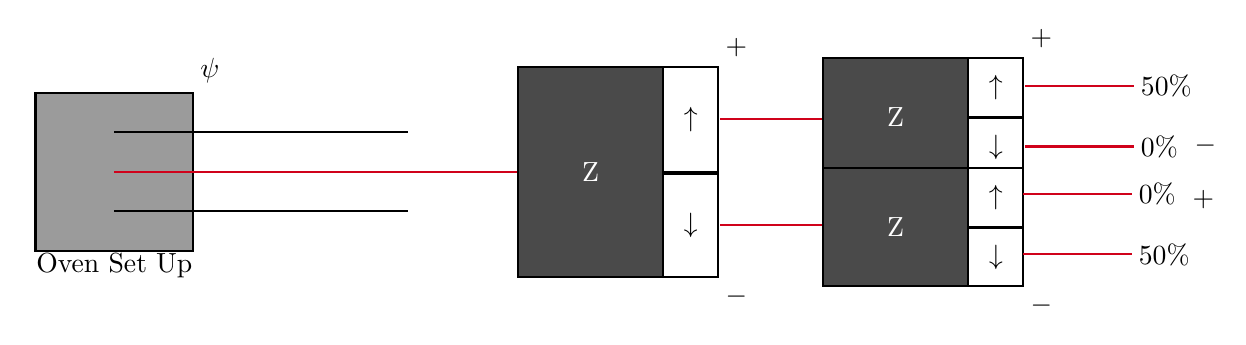
\begin{tikzpicture}[x=0.75pt,y=0.75pt,yscale=-1,xscale=1]
%uncomment if require: \path (0,375); %set diagram left start at 0, and has height of 375

%Shape: Square [id:dp14421103605944618] 
\draw  [fill={rgb, 255:red, 155; green, 155; blue, 155 }  ,fill opacity=1 ] (64,128) -- (140,128) -- (140,204) -- (64,204) -- cycle ;
%Straight Lines [id:da6727148484422872] 
\draw [color={rgb, 255:red, 208; green, 2; blue, 27 }  ,draw opacity=1 ]   (243.42,166) -- (102,166) ;
%Shape: Rectangle [id:dp31052784363324215] 
\draw  [fill={rgb, 255:red, 74; green, 74; blue, 74 }  ,fill opacity=1 ] (296.42,115.36) -- (366.42,115.36) -- (366.42,216.64) -- (296.42,216.64) -- cycle ;
%Straight Lines [id:da9714115391207371] 
\draw    (243.42,147) -- (102,147) ;
%Straight Lines [id:da9565511475124852] 
\draw    (243.42,185) -- (102,185) ;
%Straight Lines [id:da5775689584288694] 
\draw [color={rgb, 255:red, 208; green, 2; blue, 27 }  ,draw opacity=1 ]   (295.84,166) -- (243.42,166) ;
%Shape: Rectangle [id:dp34780699384586333] 
\draw  [fill={rgb, 255:red, 255; green, 255; blue, 255 }  ,fill opacity=1 ] (366.42,167) -- (393,167) -- (393,216.64) -- (366.42,216.64) -- cycle ;
%Shape: Rectangle [id:dp9674012952324293] 
\draw  [fill={rgb, 255:red, 255; green, 255; blue, 255 }  ,fill opacity=1 ] (366.42,115.36) -- (393,115.36) -- (393,166) -- (366.42,166) -- cycle ;
%Straight Lines [id:da8039050506004896] 
\draw [color={rgb, 255:red, 208; green, 2; blue, 27 }  ,draw opacity=1 ]   (446.13,140.68) -- (393.71,140.68) ;
%Straight Lines [id:da5371523365899473] 
\draw [color={rgb, 255:red, 208; green, 2; blue, 27 }  ,draw opacity=1 ]   (446.13,191.82) -- (393.71,191.82) ;
%Shape: Rectangle [id:dp5066877735662358] 
\draw  [fill={rgb, 255:red, 74; green, 74; blue, 74 }  ,fill opacity=1 ] (443.42,111.36) -- (513.42,111.36) -- (513.42,168) -- (443.42,168) -- cycle ;
%Shape: Rectangle [id:dp7068517018359358] 
\draw  [fill={rgb, 255:red, 255; green, 255; blue, 255 }  ,fill opacity=1 ] (513.42,140.24) -- (540,140.24) -- (540,168) -- (513.42,168) -- cycle ;
%Shape: Rectangle [id:dp5547396655118183] 
\draw  [fill={rgb, 255:red, 255; green, 255; blue, 255 }  ,fill opacity=1 ] (513.42,111.36) -- (540,111.36) -- (540,139.68) -- (513.42,139.68) -- cycle ;

%Straight Lines [id:da925156022518015] 
\draw [color={rgb, 255:red, 208; green, 2; blue, 27 }  ,draw opacity=1 ]   (593.13,124.68) -- (540.71,124.68) ;
%Straight Lines [id:da995628624290608] 
\draw [color={rgb, 255:red, 208; green, 2; blue, 27 }  ,draw opacity=1 ]   (593.13,153.82) -- (540.71,153.82) ;
%Shape: Rectangle [id:dp6769071252491495] 
\draw  [fill={rgb, 255:red, 74; green, 74; blue, 74 }  ,fill opacity=1 ] (443.42,164.36) -- (513.42,164.36) -- (513.42,221) -- (443.42,221) -- cycle ;
%Shape: Rectangle [id:dp6306771616992262] 
\draw  [fill={rgb, 255:red, 255; green, 255; blue, 255 }  ,fill opacity=1 ] (513.42,193.24) -- (540,193.24) -- (540,221) -- (513.42,221) -- cycle ;
%Shape: Rectangle [id:dp43240360470130335] 
\draw  [fill={rgb, 255:red, 255; green, 255; blue, 255 }  ,fill opacity=1 ] (513.42,164.36) -- (540,164.36) -- (540,192.68) -- (513.42,192.68) -- cycle ;

%Straight Lines [id:da3774129227180918] 
\draw [color={rgb, 255:red, 208; green, 2; blue, 27 }  ,draw opacity=1 ]   (592.13,176.68) -- (539.71,176.68) ;
%Straight Lines [id:da9566074019333357] 
\draw [color={rgb, 255:red, 208; green, 2; blue, 27 }  ,draw opacity=1 ]   (592.13,205.82) -- (539.71,205.82) ;

% Text Node
\draw (102,204) node [anchor=north] [inner sep=0.75pt]   [align=left] {\begin{minipage}[lt]{61.13pt}\setlength\topsep{0pt}
\begin{center}
Oven Set Up
\end{center}

\end{minipage}};
% Text Node
\draw (331.42,166) node  [color={rgb, 255:red, 255; green, 255; blue, 255 }  ,opacity=1 ] [align=left] {Z};
% Text Node
\draw (379.71,140.68) node    {$\uparrow $};
% Text Node
\draw (379.71,191.82) node  [rotate=-180]  {$\uparrow $};
% Text Node
\draw (142,124.6) node [anchor=south west] [inner sep=0.75pt]    {$\ket{\psi }$};
% Text Node
\draw (395,111.96) node [anchor=south west] [inner sep=0.75pt]    {$\ket{+}$};
% Text Node
\draw (395,220.04) node [anchor=north west][inner sep=0.75pt]    {$\ket{-}$};
% Text Node
\draw (542,107.96) node [anchor=south west] [inner sep=0.75pt]    {$\ket{+}$};
% Text Node
\draw (542,224.4) node [anchor=north west][inner sep=0.75pt]    {$\ket{-}$};
% Text Node
\draw (478.42,139.68) node  [color={rgb, 255:red, 255; green, 255; blue, 255 }  ,opacity=1 ] [align=left] {Z};
% Text Node
\draw (526.71,125.52) node    {$\uparrow $};
% Text Node
\draw (526.71,154.12) node  [rotate=-180]  {$\uparrow $};
% Text Node
\draw (595.13,124.68) node [anchor=west] [inner sep=0.75pt]    {$50\%$};
% Text Node
\draw (595.13,153.82) node [anchor=west] [inner sep=0.75pt]    {$0\%$};
% Text Node
\draw (526.71,207.12) node  [rotate=-180]  {$\uparrow $};
% Text Node
\draw (526.71,178.52) node    {$\uparrow $};
% Text Node
\draw (478.42,192.68) node  [color={rgb, 255:red, 255; green, 255; blue, 255 }  ,opacity=1 ] [align=left] {Z};
% Text Node
\draw (594.13,176.68) node [anchor=west] [inner sep=0.75pt]    {$0\%$};
% Text Node
\draw (594.13,205.82) node [anchor=west] [inner sep=0.75pt]    {$50\%$};
% Text Node
\draw (620,185.28) node [anchor=south west] [inner sep=0.75pt]    {$\ket{+}$};
% Text Node
\draw (621,147.4) node [anchor=north west][inner sep=0.75pt]    {$\ket{-}$};


\end{tikzpicture}
